\documentclass[11pt]{beamer}
\usepackage[utf8]{inputenc}
\usepackage[T1]{fontenc}
\usepackage{amsmath}
\usepackage{amsfonts}
\usepackage{amssymb}
\usepackage{graphicx}
\usetheme{default}

\begin{document}
	\author{Musa Baloyi}
	\title{Elasticsearch for Hadoop}
	%\subtitle{Model governance for risk management}
	%\logo{}
	%\titlegraphic{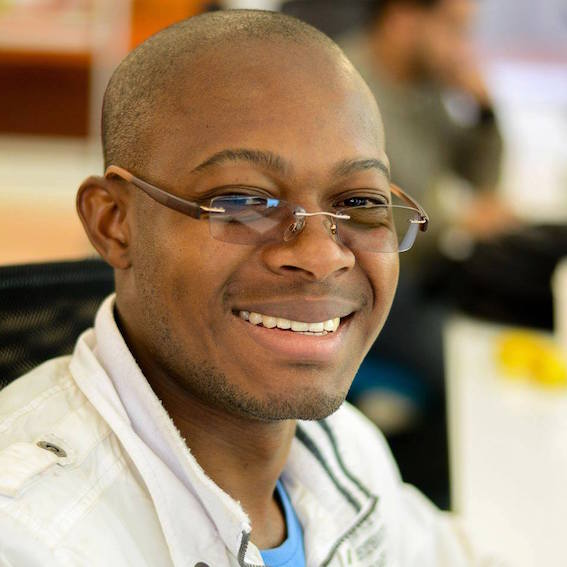
\includegraphics[width=\textwidth,height=.5\textheight]{logo}}
	%\institute{}
	%\date{}
	%\subject{}
	%\setbeamercovered{transparent}
	%\setbeamertemplate{navigation symbols}{}
	\begin{frame}[plain]
	\maketitle
\end{frame}

\begin{frame}
\frametitle{Table of contents}
\begin{itemize}
	\item Elasticsearch for Hadoop
	\item Architectural overview
	\item Kafka
	\item Gobblin
	\item Confluent
\end{itemize}
\end{frame}


\begin{frame}
\frametitle{Elasticsearch for Hadoop}
\begin{figure}[h]
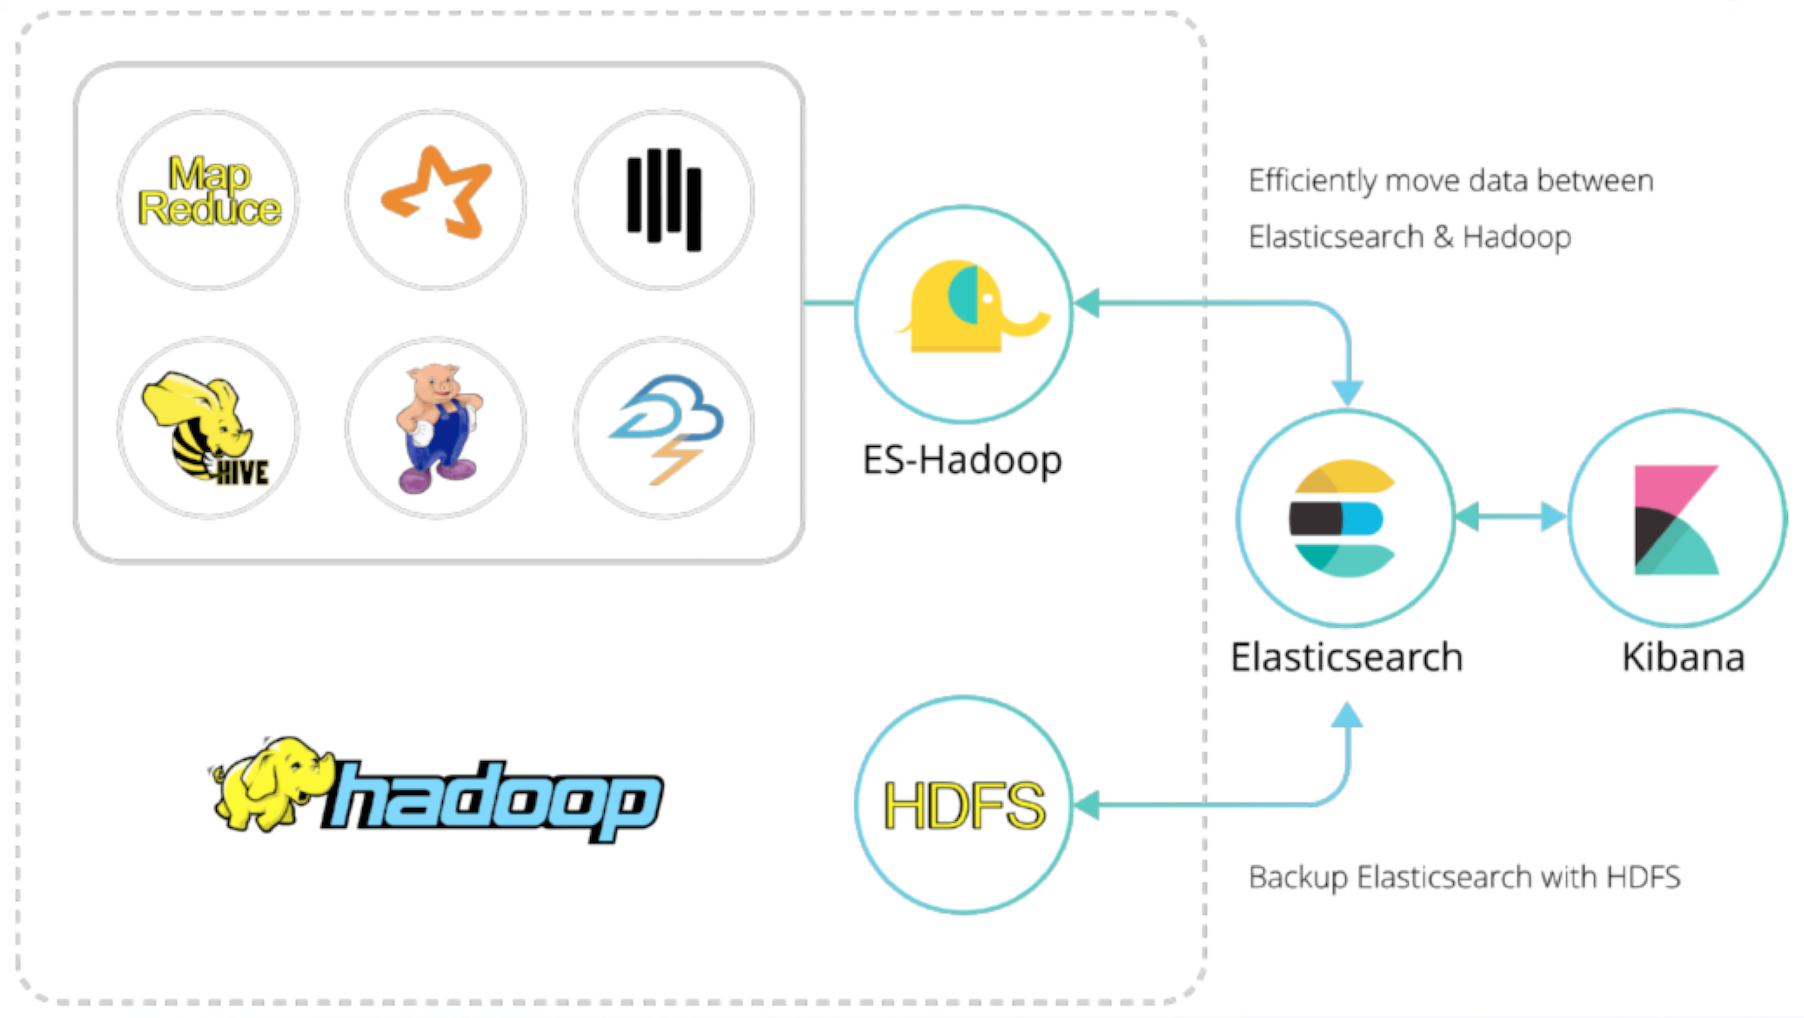
\includegraphics[scale=.3]{images/es_hdp}
\end{figure}
\end{frame}

\begin{frame}
\frametitle{Architectural overview (previous vision)}
\begin{figure}[h]
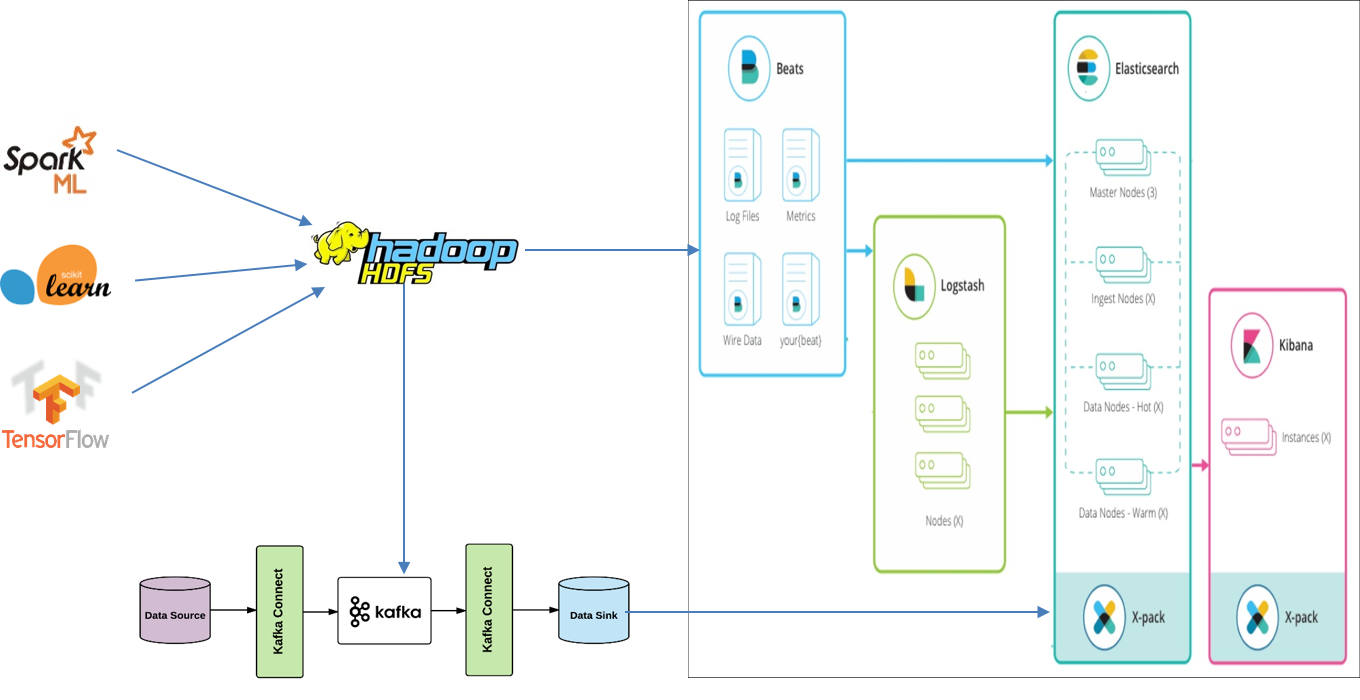
\includegraphics[scale=.3]{images/arch1}
\end{figure}
\end{frame}

\begin{frame}
\frametitle{Architectural overview (***NEW***)}
\begin{figure}[h]
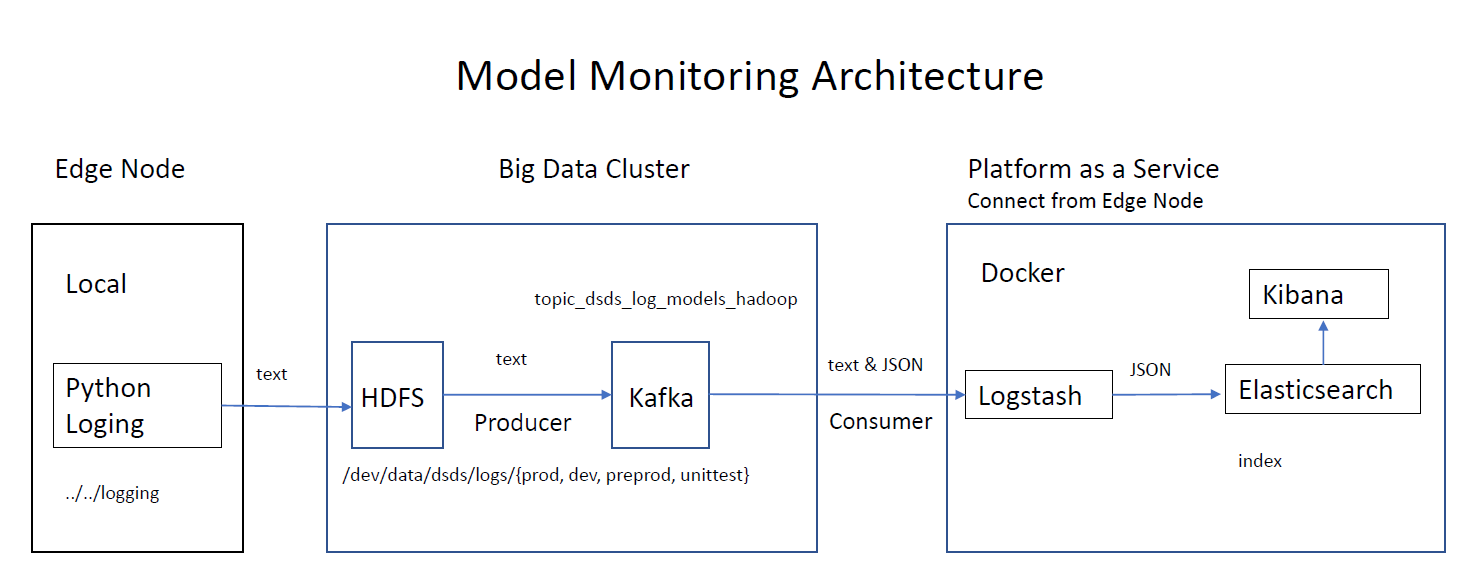
\includegraphics[scale=.25]{images/arch2}
\end{figure}
\end{frame}

\begin{frame}
\frametitle{Architectural overview (current)}
\begin{figure}[h]
	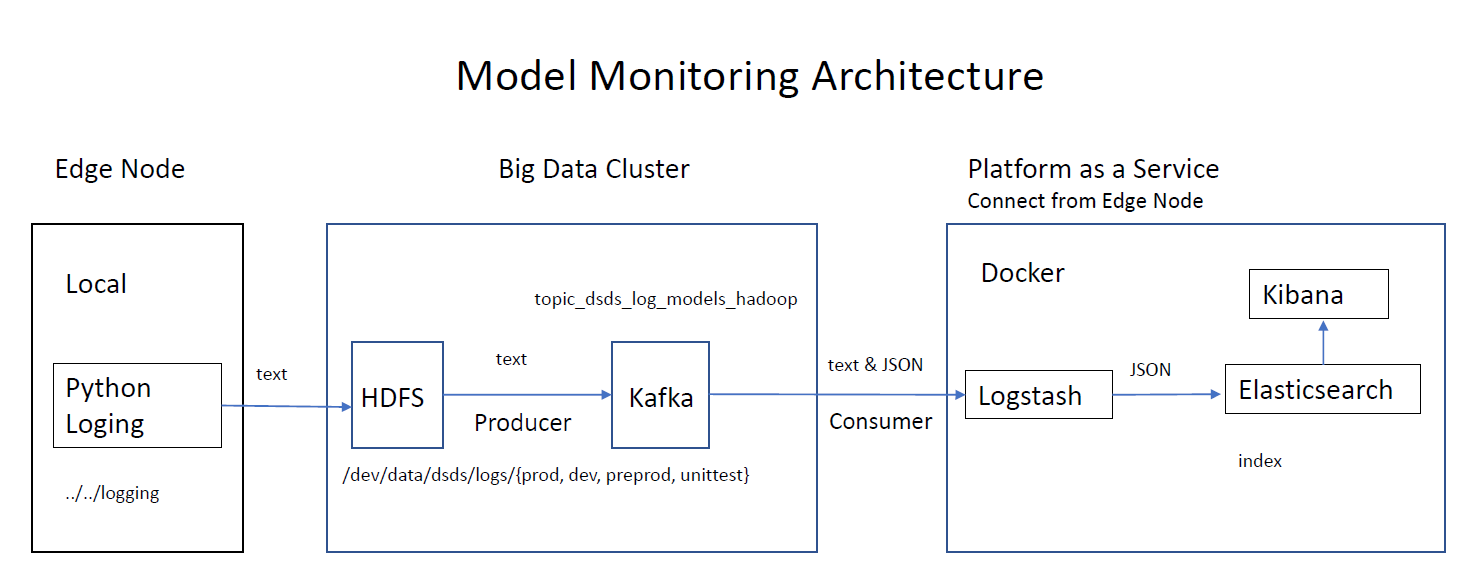
\includegraphics[scale=.25]{images/arch2}
\end{figure}
\end{frame}

\begin{frame}
\frametitle{Kafka}
\begin{itemize}
\item Kafka is generally used for building real-time streaming 
\begin{itemize}
\item data pipelines that reliably get data between systems or applications
\item applications that transform or react to the streams of data
\end{itemize}
\item Kafka is run as a cluster on one or more servers that can span multiple datacenters.
\item The Kafka cluster stores streams of records in categories called topics.
\item Each record consists of a key, a value, and a timestamp.
\end{itemize}
\end{frame}

\begin{frame}
\frametitle{Kafka installation}
\begin{itemize}
\item Download the binary: kafka\_2.12-1.0.1.tgz 
\item 7z x  kafka\_2.12-1.0.1.tgz \&\& 7z x  kafka\_2.12-1.0.1.tar
\item sudo mv kafka\_2.12-1.0.1 /opt/Kafka
\end{itemize}
\end{frame}

\begin{frame}
\frametitle{Kafka demo}
\begin{itemize}
\item cd /opt/Kafka/ kafka\_2.12-1.0.1
\item sudo bin/kafka-server-start.sh config/server.properties
\item bin/kafka-console-consumer.sh --bootstrap-server localhost:9092 --topic testing --from-beginning
\item bin/kafka-topics.sh --create --zookeeper localhost:2181 --replication-factor 1 --partitions 1 --topic testing
\item bin/kafka-topics.sh --list --zookeeper localhost:2181
\item Configure Kafka producer connect-file-source.properties
\item Configure Kafka consumer connect-file-sink.properties
\item bin/connect-standalone.sh config/connect-standalone.properties config/connect-file-source.properties config/connect-file-sink.properties
\end{itemize}
\end{frame}


\begin{frame}
\frametitle{References}
\begin{enumerate}
\item Building Intelligent Systems: A Guide to Machine Learning Engineering. [Geoff Hulten] (Apress, 2018)
\item Trends in AI, Data Science, and Big Data. [Ben Lorica] (2017)
\item Building Evolutionary Architectures. [Rebecca Parsons; Patrick Kua; Neal Ford] (O'Reilly Media, 2017)
\item 5 things you should be monitoring. [Brian Brazil] (2018)
\item The Logstash Book. [James Turnbull] (Turnbull Press, 2013)
\item Beyond the Twelve-Factor App. [Kevin Hoffman] (O'Reilly Media, 2016)
\item Logs and real-time stream processing. [Jay Kreps] (2016)
\item I Heart Logs: Apache Kafka and Real-time Data Integration. [Jay Kreps] (2015)
\item The log: The lifeblood of your data pipeline. [Kiyoto Tamura] (2015)
\item Understanding the ELK stack. [Brian Anderson; Rafał Kuć] (2016)
\end{enumerate}
\end{frame}

\end{document}